\documentclass{article}

% Package imports
\usepackage{titlesec}
\usepackage{geometry}
\usepackage{fancyhdr}
\usepackage{graphicx}
\usepackage{hyperref} % \url, https://www.overleaf.com/learn/latex/Hyperlinks
\usepackage{outlines} % better itemize
\usepackage{comment}
\usepackage{multirow} % tables
\usepackage{noto} % Google Noto Fonts
\usepackage{hyperref} % Hyperlinks to sectiosn

\usepackage[british]{datetime2} % load before gitinfo2 to customize
\usepackage[mark=true,grumpy=true]{gitinfo2}

% Redefine \gitMark to customize it
% https://mirror.apps.cam.ac.uk/pub/tex-archive/macros/latex/contrib/gitinfo2/gitinfo2.pdf
\renewcommand{\gitMark}{Branch: \gitBranch\,@\,\gitAbbrevHash{}\,\textbullet{}\,\DTMusedate{gitdate}}

\geometry{a4paper, includeheadfoot, portrait, total={}, top=12.5mm, bottom=12.5mm, left=12.5mm, right=12.5mm}

\graphicspath{ {./images/} }

% Variables
\def\projectname{Inventory Project}

% Override subparagraph with a variant that has no indentation
% https://tex.stackexchange.com/a/392014
\makeatletter
\renewcommand\subparagraph{%
\@startsection{subparagraph}{5}{0pt}%
{3.25ex \@plus 1ex \@minus .2ex}{-1em}%
{\normalfont\normalsize\bfseries}}
\makeatother

\title{\projectname}
\author{James Cahill}
\date{Sepetember 2023}

% Configure fancyHDR page style
% https://tex.stackexchange.com/questions/266911/get-fancyhdr-and-geometry-to-work-nicely
\fancypagestyle{style}{
    \fancyhead{} % clear all header fields
    \fancyhead[HL]{\projectname}
    \fancyhead[HR]{James Cahill}
    \renewcommand{\headrulewidth}{0pt} % Remove header line
}
\pagestyle{style}


\begin{document}


\tableofcontents

\pagebreak

\section{Analysis}

% Background
\subsection{Problem Identification}

\subsubsection{Problem Description}

\begin{comment}
    - not always designed for multi user?
    - not intuitive?

    GS (till end): not user friendly?
    shoudn't be time consuming to add data/etc
    manual admin can be time consuming, try to automate
    ability for mutliple concurrent users
        easy and transpaancy for multi users
                log in and see what was done the day before
                    easy to follow/read

    not able to re-order items in a single place
    have to go do diff platforms when ready to re-order

    limited functionality
        want to be able to track purchased items
        as well as handle budgeting
        existing solutions don't have multiple functions
        so you need to duplicate information on different apps/areas
        like how Monzo combines budgeting with card and tracking txns.

    are these a problem with the current app or a problem you have that
    you need a solution to.

    is problem with current app
    or need support with inventory/organisation

    do more research on downsides of different alternatives/
\end{comment}

Popular inventory management solutions are relatively expensive, and may be out
of reach for individuals or small schools.
Inventory systems have numerous benefits for businesses and individuals alike; a business
may choose to track their supply levels where an individual may wish to catalogue their DVD collection. \\

\noindent My goal is to create a web-based application aimed at both businesses and individuals to manage
inventory, with additional modern features such as automatic item re-ordering when stocks are running low.\\

\noindent Traditional inventory management solutions are typically single-user at best, whereas I intend to create
a multi-user, collaborative environment.\\

\noindent In my view, an inventory system should be:

\begin{outline}
    \1 Easy for end users to use.
    \1 Cross platform
    \1 Performant interface
    \1 Efficient in terms of adding data
    \1 Allow for easy cataloguing of inventory
    \1 Allow for item scanning using QR codes / barcodes
    \1 Be able to source data from external sources
    \1 Support both consumable and non-consumable goods.

    
\end{outline}


\begin{comment}
An inventory system should be able to:

time consuming to add data
not user friendly

- catalogue of inventory, re-order for you
- scan using a phone (no external hardware needed)
- alert / re-order when stocks are running low.
- purchase links
- stretch: source data from amazon or equivalent instead of typing it manually
- search engine for catalogued and new Parts
    - provides with options for where to purchase certain goods
- button to re-order
    - smart device???????
- predict when stocks will run out.
- source data from external sources
- like monzo projection of when it will run out
- how much you are spending each month on goods
- nfc support to easily scan / etc items (might be too hard on iOS)
\textbf{Barcode check in / out}
- monzo integration
- budgeting - figure projections  as well 
clearly define what the APP will feature.
Think about
- potential users
    - how does the app cater to their needs - different features etc


\end{comment}

\subsubsection{Stakeholders}

Stakeholder requirements are further discussed for each stakeholder in the \underline{\hyperref[sec:stakeholderRequirements]{Stakeholder Requirements}} section.\\

\newcommand{\stakeholderEntry}[4]{{#1} & {#2} & {#3} & {#4}\\\hline}

\begin{tabular}{ |p{0.15\textwidth}|p{0.26\textwidth}|p{0.26\textwidth}|p{0.26\textwidth}| }
    \hline
    \textbf{Stakeholder} & \textbf{Description} & \textbf{Requirements} & \textbf{Capability}\\
    \hline

    \stakeholderEntry
        {Claire Foley}
        {Senior Leadership Team at The Village Prep School}
        {Ability to manage library books. Admin and supervision of other users carrying out librarian tasks}
        {Well-versed in computer use, at least when it comes to intuitive and well designed interfaces. Would struggle with a non-intuitive interface design.}
    
    \stakeholderEntry
        {Ella}
        {"Head Librarian" (Pupil) at the Village Prep School}
        {Ability to check in and out library books. User of the system; requires interface that is appropriate for her age.}
        {Beginner user of technology, proficient in mobile applications on phones and tablets only. Rarely uses a laptop or desktop computer.}
    
    \stakeholderEntry
        {Generic Gear \newline Rental Shop}
        {Photography gear for hire business}
        {Ability to manage business inventory in a fast and efficient manner.}
        {Proficient with computers.}
    \hline
\end{tabular}


\subsubsection{Interview}

\paragraph{Question Set}
\begin{outline}
    \1 What would you consider your skill level to be regarding technology?
    \1 Do you currently have a way to manage inventory?
    \2 If so, what is your current solution?
    \3 What aspects of this solution do you like?
    \3 What aspects of this solution do you dislike?
    \2 What features would you \textbf{require} in a custom solution?
    \2 What features would \textbf{enchance} your experience?
\end{outline}

\begin{comment}
    CF 
CF "SLT": library

    what is the current system?
        borrowing cards and date stamps that are manually written in for when books are due back
        borrower card for who borrowed which book, stickers placed on books for categories

    problems with existing solution
        time consuming; cards get lost; stickers fall off
        not very quick to see who borrowed what; have to look through all cards
        
    
    like about the existing solution
        primary aged students/children can do it (themselves)
    
    requirements for new solution

        scan a barcode / borrower ticket and instantly see what they've borrowed.
        
        cost effective
        compatible with existing hardware/software
        works on ipa
        ability to renew
        notified when books are overdue
        statistics (book numbers) by genre/author/category
    
    enhancements for new solution
        colored stickers for categories
        ability to charge parents (make an invoice?)
    
    is there a specific way you would like the system to be organised?
        yes, we are a library so by preset genres and categories
    
    do you have any questions of your own?
        what's the timeframe for this being completed - March.

fake pupil: Ella (no surname)
year 6 "head librarian" age 10-**11** (y6)

    problems with the current system
        "so old fashioned, should be able to scan using my iPad! Then it could be pupil-led."
    
    benefits
        can see who borrowed the book I want and nag them to return it so I can read it!
        when I forget which book I've borrowed the teacher can easily find which books I've lost
    
    requirements
        iPads; fast (can be done in break times - borrow/renew)
    
    
        

fake teacher
equipment for science lab/art room/ etc


can say helping a junior school.

    
\end{comment}

\pagebreak

\subsubsection{Existing similar solutions}

% do 4-5 alternatives

% 1. InvenTree
\paragraph{\\InvenTree}
\url{https://inventree.org/}

\subparagraph{\\Overview\\}

InvenTree is an \textbf{open-source} inventory management system, providing \textit{low level stock control and part tracking}.
It uses a Python/Django database backend and provides both a \textbf{web-based interface} as well as a REST API for interacting with other services.
InvenTree also has a powerful plugin system for custom applications and other extensions. \\

\noindent Below is a screenshot of the InvenTree homepage.\\
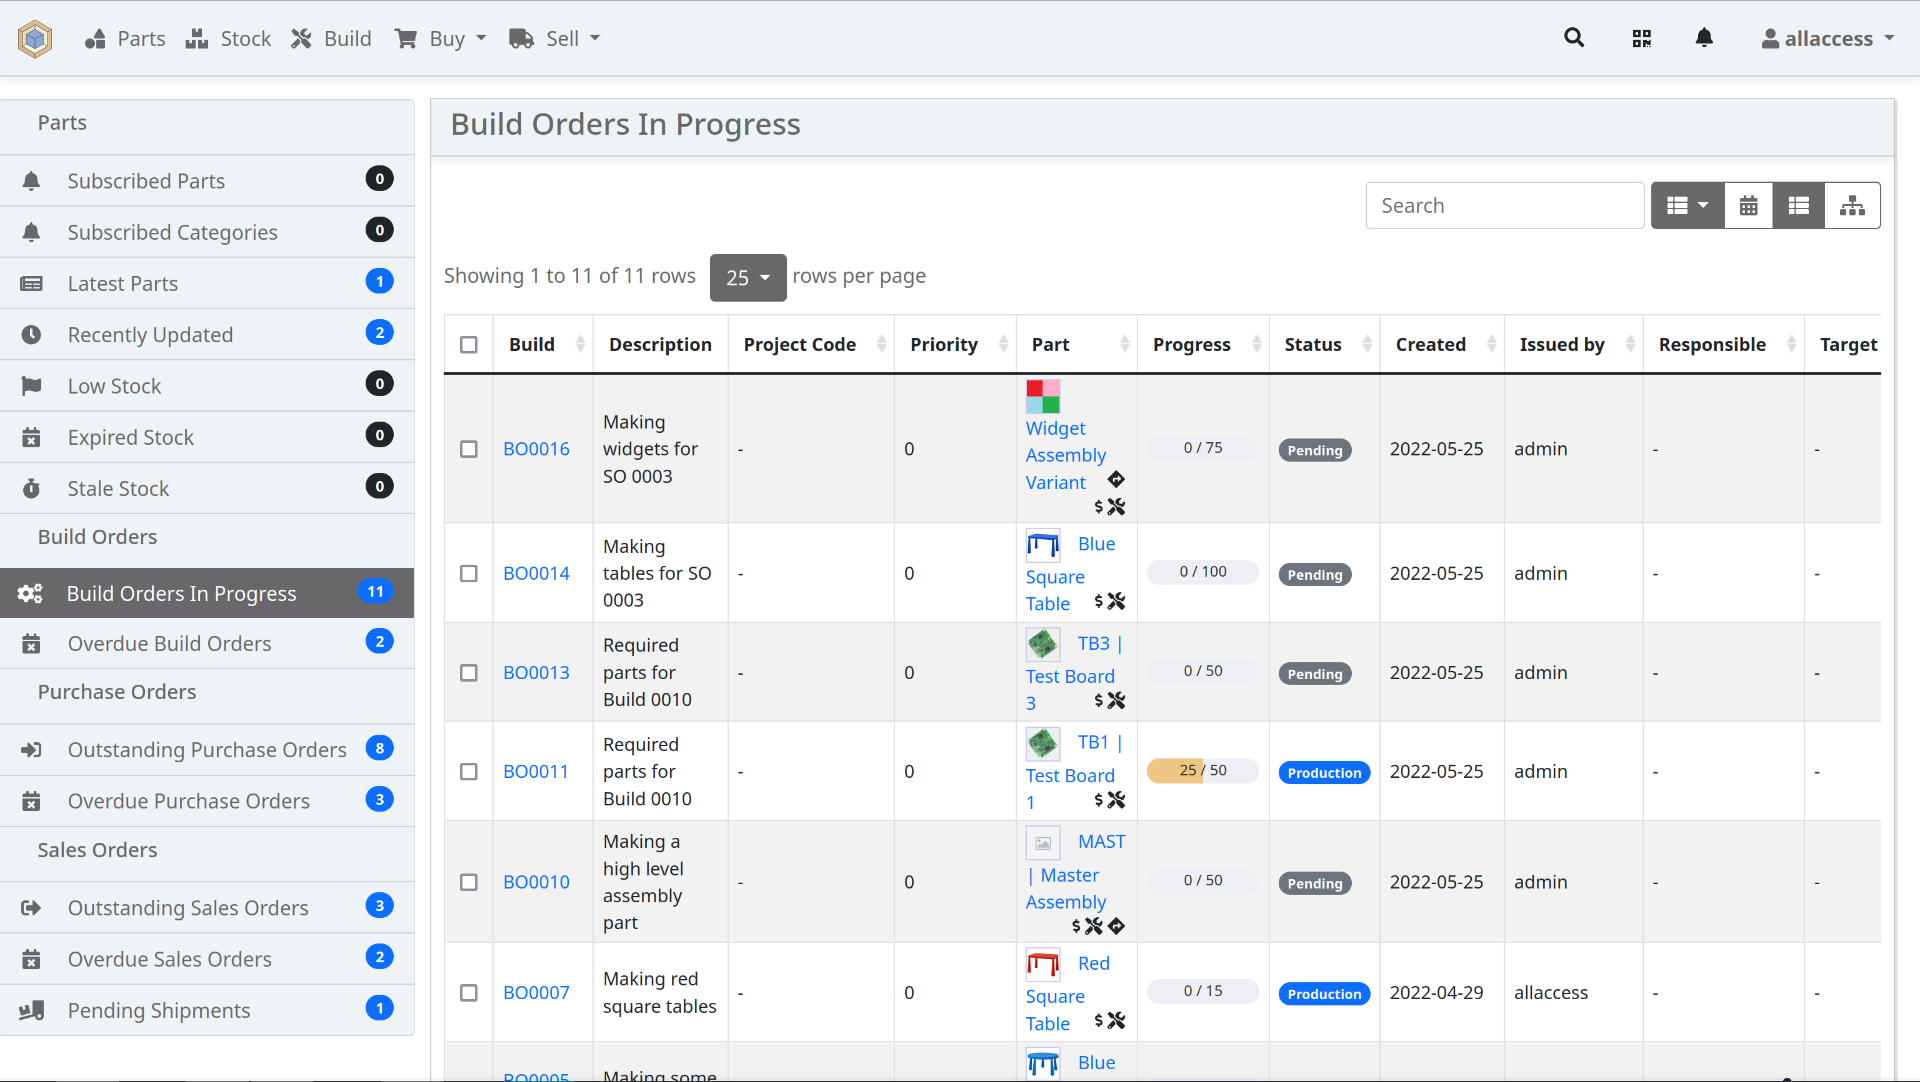
\includegraphics[width=15cm]{inventree_demo_homepage.png}

\subparagraph{Parts applicable to my solution\\}

The core concept is similar (the application is web-based), but my solution will be more generalized that just stock control.

\pagebreak

% 2. PartKeepr
\paragraph{\\PartKeepr}
\url{https://partkeepr.org/}\\

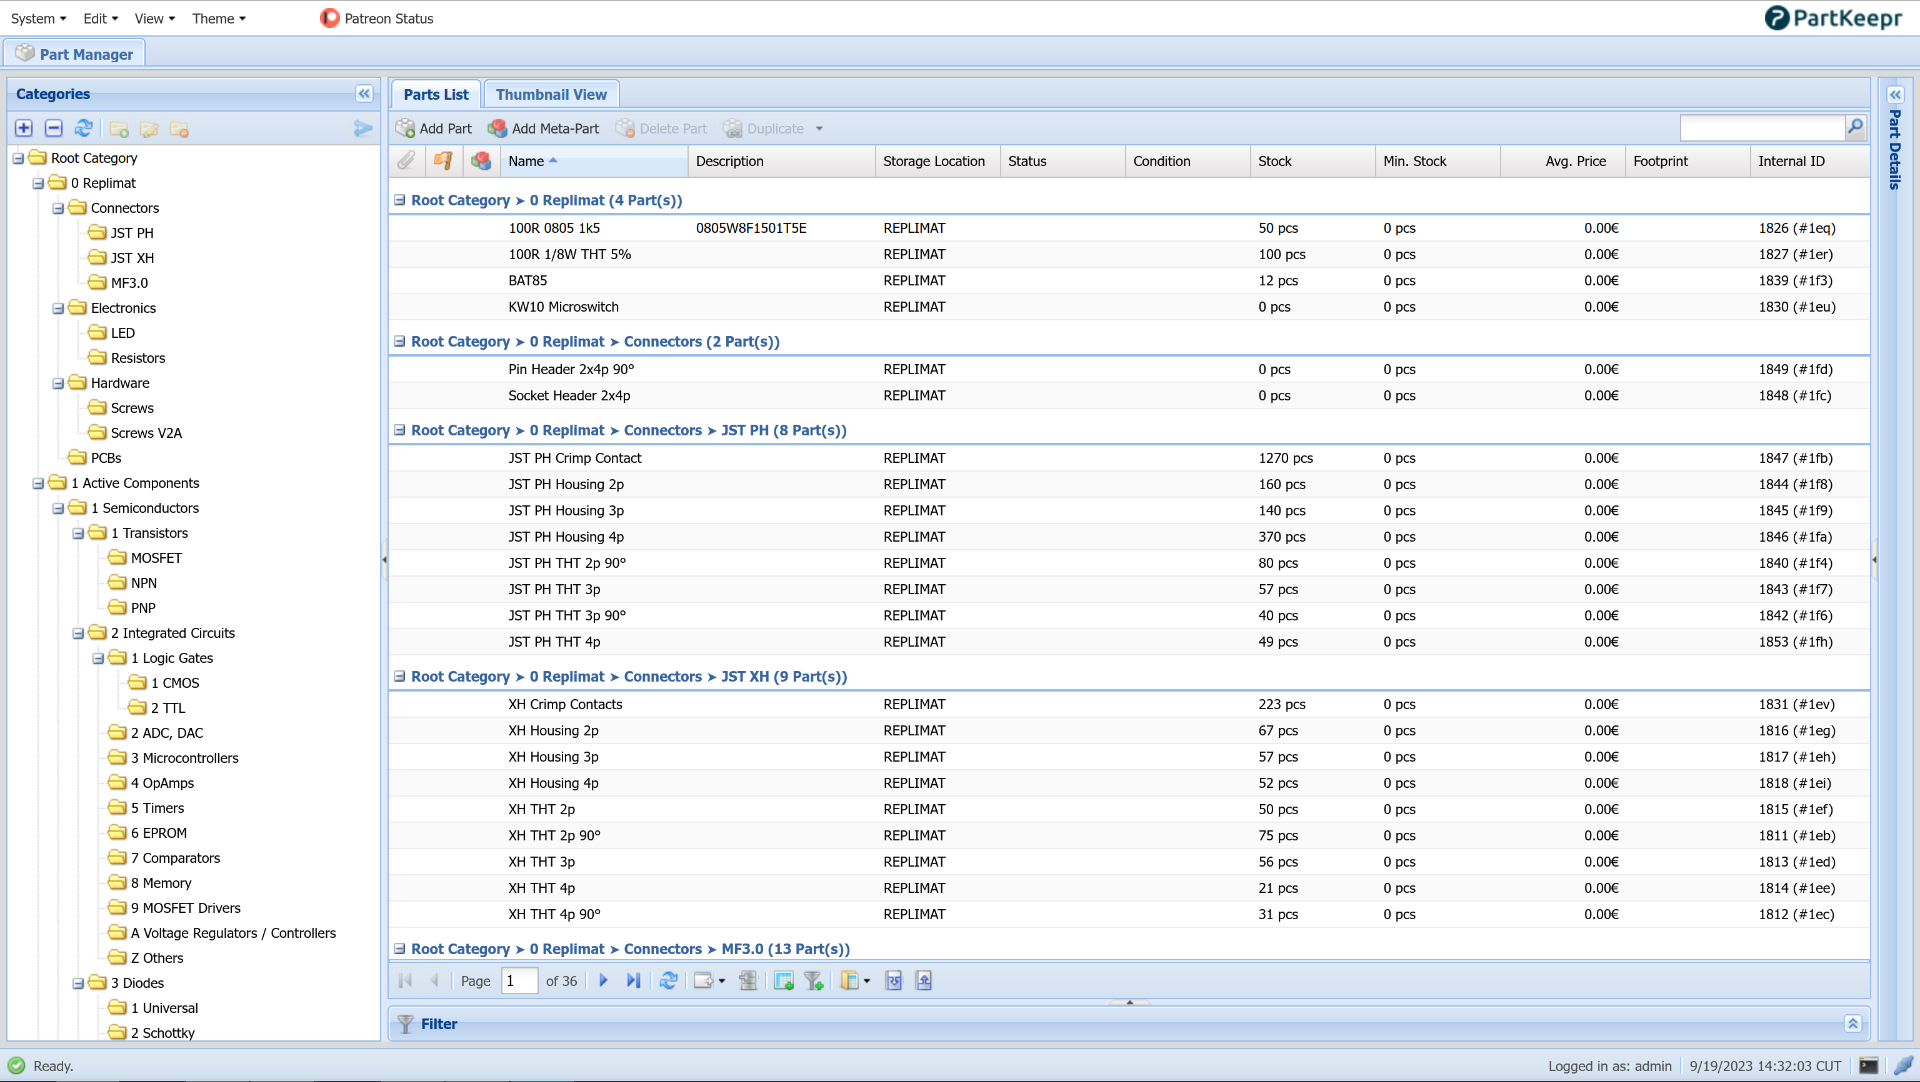
\includegraphics[width=15cm]{partkeepr_demo_homepage.png}

\subparagraph[indent=false]{\\Overview\\}

PartKeepr is an open-source inventory management system with a focus on electronic components.
It is designed around four main principles:

\begin{outline}
    \1 Fast Part Searching
    \1 Ability to add complete part database
    \1 Keeping track of stock
    \1 Ease of use
\end{outline}

\subparagraph{Parts applicable to my solution\\\\}

\noindent Like PartKeepr, I hope to implement a web-based interface.
However, I am using a different approach as my solution will not be tailored specifically to electronic components.

\pagebreak

% 3. Sortly
\paragraph{\\Sortly}
\url{https://www.sortly.com/solutions/inventory-management-software/}\\

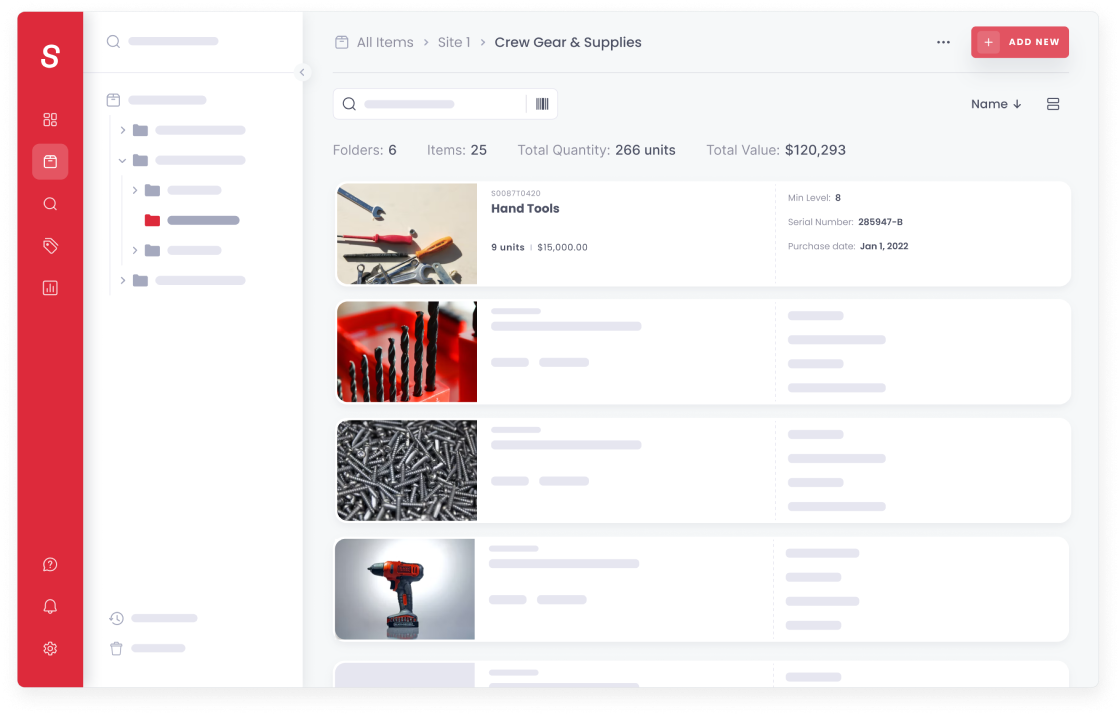
\includegraphics[width=15cm]{sortly_homepage_mockup_1.png}

\subparagraph{\\Overview\\}

Sortly is a proprietary cloud-based inventory management system with a focus on small businesses and inviduals.\\\\
It has two plans available, an always free plan with limited functionality and a paid plan will a more complete feature-set.

\subparagraph{Parts applicable to my solution\\\\}

I hope to implement the following features from Sortly:

\begin{outline}
    \1 Web based interface
    \2 Allows for easy access.

    \1 Barcode support
    \2 Allows end users to print off QR codes to stick to items
    \2 Which can be scanned in-app to easily perform actions on the item.

    \1 Real-time reporting insights
    %\subitem 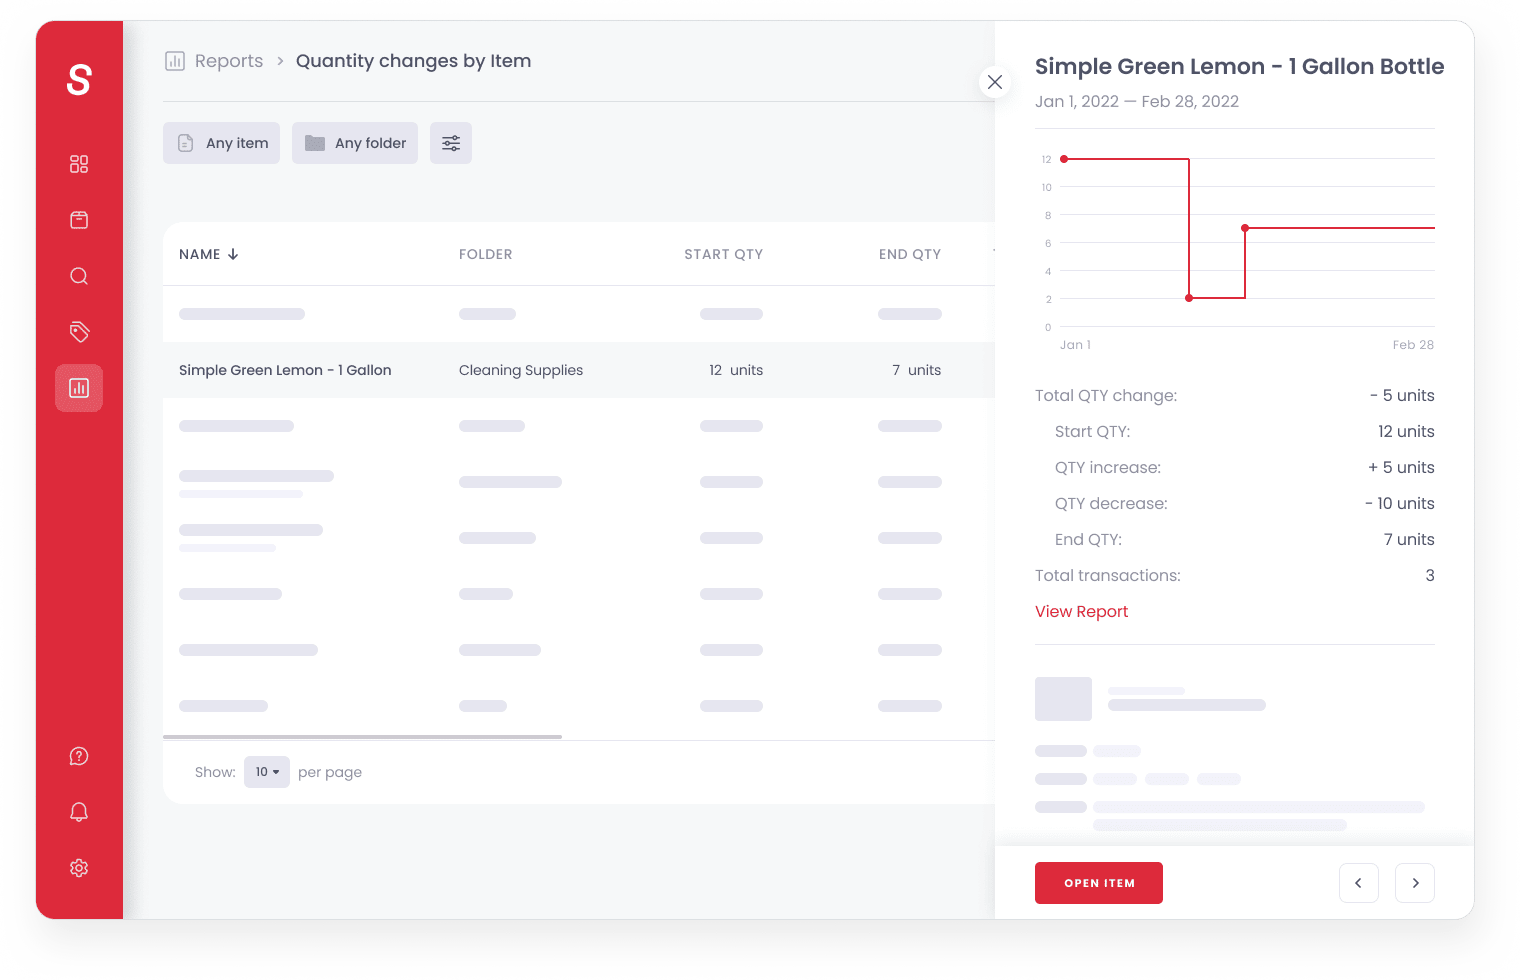
\includegraphics[width=10cm]{sortly_homepage_mockup_2.png}
    \2 Allows for added insight into usage patterns for particular units.
\end{outline}

\subsubsection{Features to be incorporated into solution}

\subsubsection{Feedback from stakeholders}

\subsection{Requirements}

\subsubsection{Stakeholder requirements}
\label{sec:stakeholderRequirements}

\pagebreak

\subsubsection{Software and hardware requirements}

\paragraph{System Requirements\\\\}

\begin{tabular}{ |p{0.45\textwidth}|p{0.5\textwidth}| }
    \hline
    \textbf{Hardware} & \textbf{Justification}\\
    \hline
    \textit{Laptop/Desktop}\newline
    Keyboard and Pointing Device (eg. Mouse) &
    For desktop or laptop computer users, a suitable input device is required in order to interact with the software.\newline
    A pointing device (a mouse) is necessary in order to interact with the user interface, to perform actions such as clicking buttons, icons, and opening menus.\newline
    A keyboard will be used to manually input data into the system.\\
    \hline
    \textit{Tablet Device}\newline
    Touchscreen & For tablet users, it would be impractical to expect the user to have access to a keyboard and or pointing device. Therefore, we must design the system to accept inputs from a touchscreen.\newline
    This will be easier to use and more intuitive for tablet users. \newline
    The touchscreen will be used to input data into the system and to interact with the user interface. \\
    \hline
    Dual-Core Processor
    \newline(x86, ARM, RISCV architectures) &
    A modern processor with sufficient resources to run an up-to-date web browser such as Chrome, Edge or Firefox is required in order to access the web-based interface.\\
    \hline
    2GB of RAM & Sufficient RAM is required to run the web browser, which can be a memory intensive task.\\
    \hline
    Monitor & To display the user interface. \\
    \hline
    Network Interface Card (NIC) & A Network Interface Card, or NIC, is required for the computer to be connected to a network, such as the Internet. This is required as the web interface will be hosted on a domain and server that is external to the user, that is to say, not on their local network. \\
    \hline
    \textit{\textbf{Optional}: Wireless Network Adapter} & \textit{A Wireless Network Adapter is an optional requirement, it will allow the user to connect to a wireless network in order to access the network or Internet so that they can access the external user interface.} \\
    \hline
    \textit{\textbf{Optional}: Camera} & \textit{A Camera is an optional requirement; devices with cameras will be able to scan barcodes or QR codes corresponding to inventory items and easily perform actions on them.} \\
    \hline
\end{tabular}

\paragraph{Software Requirements\\\\}

Talk about why I don't need much software since dependencies hosted on the server.\\

\begin{tabular}{ |p{0.45\textwidth}|p{0.5\textwidth}| }
    \hline
    \textbf{Software} & \textbf{Justification}\\
    \hline
    Operating System \newline
    \textit{(Windows, MacOS, Linux, ChromeOS, iOS, iPadOS, Android)} &
    An operating system is required in order to run the web browser necessary to access the interface. \\
    \hline
    A web browser \newline
    \textit{(eg. Chrome, Firefox, Microsoft Edge, Safari)} &
    A web browser is necessary to access the interface as it will be primarily a web application.\\
    \hline
\end{tabular}

\pagebreak

\subsubsection{Success requirements}

The overall objectives for the system.

\noindent To measure the overall effectiveness of the system, targets must be set before writing the program.
These targets will help in the evaluation stage to determine weather our objectives have been met.
These objectives will be \textbf{SMART}, i.e:

\begin{outline}
    \1 \textbf{Specific}\\
    What objective needs to be accomplished?
    \1 \textbf{Measurable}\\
    How can we quantify this objective?\\
    How will the success of this objective be measured? (quantitatively or qualitatively)
    \1 \textbf{Achievable}\\
    Is this objective achievable and realistic? If so, how to you plan to achieve them?
    \1 \textbf{Relevant}\\
    How does this objective benefit the end-users of this application as a whole?\\
    Why has this goal been set?
    \1 \textbf{Timely}\\
    Can this objective be completed within an appropriate time frame?\\
    At what stage in the software development lifecycle will you start implementing this goal?\\
    In which order will any sub-objectives be completed? 
\end{outline}

\paragraph{The Project's SMART Objectives}

\begin{enumerate}
    \item \textbf{To produce a solution for cataloguing a school library and recording users and books borrowed}\\
    At the end of the project, I will evaluate against my success criteria and determine weather this objective has been met.
    On the software side, I will be using React, Expo and PostgreSQL. This objective will be the main objective for this project.
    This objective must be completed by \underline{March 2024}.

    \item \textbf{To produce a solution including a database that can store details of books, borrowers, loans and returns}\\
    
    \item \textbf{To produce an intuitive and easy to use solution}\\
    I will evaluate my success on this objective by having a new user without any prior training or advice use the system and
    try to carry out a number of tasks without any assistance. If the user is able to successfully complete the tasks
    I will consider the system to be intuitive and easy to use and therefore this objective satisfied.
    To achieve this I will design my system to have a consistent layout based on \textbf{Material Design 2}, (\url{https://m2.material.io/})
    the design language used by Google products and many apps running on the Android operating system. I will also use language that is
    a) appropriate for the situation the product will be deployed in (with young children) and b) easy to understand (so that children can interact with the system)
    I will also use meaningful error messages so that the user has a clear understanding of the problem that has occurred.

    \item \textbf{To produce a solution that features a fully searchable catalogue}
    
    \item \textbf{To produce a solution that features reporting for overdue and/or lost books}
    \item \textbf{To produce a solution that includes a curated "suggested reading list" for each borrower}
\end{enumerate}

\begin{comment}
    GS:
        Produce a system that manages inventory in a statistical and written/informative format
        having the information automatically produce a graph
        to clearly show when stock is low

        to have a supplementary phone app that can be downloaded with the provision to
        scan and check in/out items, stored in a database.

        quantiative manner (numbers wise)
        can update a spreadsheet automatically

        able to be used remotely (T in SMART)

        data inputted to the system will be processed within a time period to produce a usable outcome
        (techy stuff goes here)

        make use of qr scanning library to easily scan QR codes that will be placed on

        display specific information about different items depending on their type
        - number of inventory available
        - highlight stock that is low
    
        predict how much you are spending on consumables
        eg. budgeting as an objective us ea library 

        asset value figure for budgeting
        are you within the budget or not
\end{comment}



\section{Design}

\subsection{User Interface Design}

\subsubsection{Usability Features}

\subsubsection{Feedback from stakeholder}

\subsection{Modular breakdown}

\subsection{Algorithms}

\subsection{Data Dictionary}

\subsection{Inputs and outputs}

\subsection{Validation}

\subsection{Testing}

\subsubsection{Methods}

\subsubsection{Test Plan}

\section{Implementation}

\subsection{First Iteration}

\section{Testing}

\section{Evaluation}

\end{document}